% vim: tw=80

\chapter{Introduction}

The field of particle physics seeks to establish a profound understanding
of the fundamental constituents of matter and the interactions between them.
The analysis of the scattering products produced in particle collisions at high
energies is an excellent method to gain deep insights into the fundamental
principles of nature.

In the endeavor to reach the highest energies in order to produce very rare
particles and to search for physics beyond our current knowledge, particle
accelerators have become ever bigger and more complex. Today's most powerful collider
is the Large Hadron Collider (LHC), where protons are accelerated to unprecedented energies. 

Protons are composed of quarks and gluons, which are referred to as partons.
The structure of the proton is described by parton distribution functions
(PDFs), which give the probability to find a quark or gluon at an
energy scale $Q$ with a fractional momentum $x$ of the proton. In contrast to
the dependence on $Q$, the $x$-dependence is not predicted by QCD but has to be parametrized and
determined from fits to experimental data. The PDFs are well constrained in the
medium $x$ region from existing measurements but exhibit a large uncertainty in
the high $x$ region which has not yet been accessible by experiments.

When the protons are brought to collision, the partons interact and produce a
plethora of new particles. These are detected and measured precisely in large
particle detectors installed around the interaction points, such as the Compact
Muon Solenoid (CMS) detector. Quarks and gluons, which are also produced
abundantly in these collisions, manifest themselves as streams of collimated
particles in the detector, the so-called particle jets. The measurement of events
containing two such jets with large transverse momenta, known as dijet events,
allows for thorough tests of predictions of Quantum Chromodynamics (QCD). The
jets are measured precisely in the CMS detector and are compared to perturbative
QCD predictions at next-to-leading order accuracy. Ultimately, insights into
the proton structure may be gained by confronting predictions with experiments
and deriving constraints on the PDFs.

In this thesis, the first measurement of triple-differential dijet cross
sections is performed at the LHC. The cross sections are measured as a function
of the average transverse momentum, the rapidity separation, and the overall
boost of the dijet pair. This triple-differential measurement separates the phase
space regions that are sensitive to the PDFs from those which are not.
Fig.~\ref{fig:intro_ybys_hint} illustrates the dijet event topologies which are
measured in this analysis:
%
\begin{itemize}
    \item The most precise dijet measurement is in the \textbf{central region}
        of the detector. For this region, the PDFs are well known and the highest transverse momenta
        of the dijets are reached. It is very well suited for the determination
        of the strong coupling constant at high energies.
    \item The \textbf{boosted region} is the most interesting for PDF studies.
        For dijets with large transverse momenta, the highest $x$ of the proton
        PDFs become accessible. Since the PDFs are not yet well known in this region,
        constraints on the PDFs can be derived from a precise
        measurement.
      \item Dijet events with a \textbf{large rapidity separation} are measured
          in the same (forward) region of the detector as the boosted dijets.
          Here, however, the probed medium-$x$ region of the PDFs is already well
          known. By considering both phase space regions in a PDF fit and exploiting the
          correlations between them, PDF and detector effects
          can be disentangled.
\end{itemize}
%
\begin{SCfigure}[][h!tp]
    \setlength{\abovecaptionskip}{5pt plus 3pt minus 2pt}
    \centering
    \caption[Illustration of dijet topologies in the various \ystar and \yboost bins]{
             Illustration of dijet event topologies measured in the different
             phase space bins. The most precise dijet measurement is in the
             central region of the detector. For PDF studies, the boosted region
             is the most interesting, since the highest $x$ of the proton are
             accessed. By exploiting the correlations between the bins with
             dijet events that exhibit a large rapidity separation and the ones
             with a large
             boost, PDF and detector effects can be disentagled.}
    \label{fig:intro_ybys_hint}
    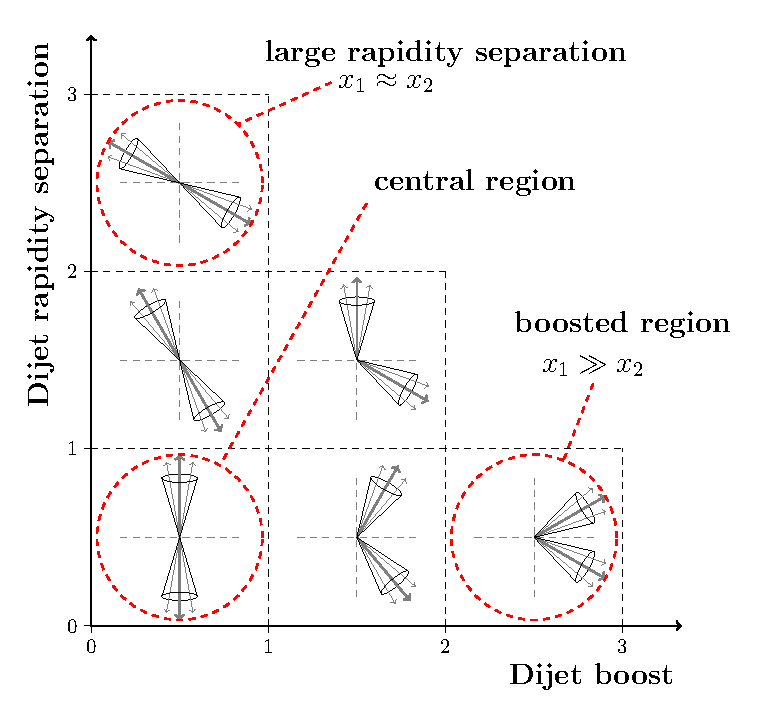
\includegraphics[width=0.5\textwidth]{figures/drawings/ybys_hint.pdf}
\end{SCfigure}
%
This thesis is structured as follows: In
Chapter~\ref{sec:theoretical_foundations}, the theoretical foundations for dijet
production at hadron colliders are outlined. An overview of the Standard Model
of particle physics with focus on perturbative QCD is given. Furthermore, the
relativistic kinematics of dijet production are explained.
Chapter~\ref{sec:experimental_setup} summarizes the experimental setup of the
CMS detector and the measurement and reconstruction of jets. 

The definition of the observables as well as the NLO calculations are discussed
in Chapter~\ref{sec:theory_predictions}. The measurement of the
triple-differential dijet cross section is presented in
Chapter~\ref{sec:measurement}. A multitude of detector and reconstruction
effects are carefully studied and related uncertainties are determined. The
measured cross sections, corrected for detector effects in an iterative
unfolding procedure, are compared to perturbative QCD calculations at NLO
accuracy. The analysis is finalized in Chapter~\ref{sec:pdf_constraints} with
studies of the PDFs. Constraints on the proton PDFs are presented. In addition,
a simultaneous fit of the PDFs and the strong coupling constant is performed.

